

\documentclass[conference]{IEEEtran}
\usepackage{color}
\usepackage{hyperref}
\usepackage{graphicx}
\usepackage{lmodern}
\usepackage{epstopdf}
\usepackage{biblatex} 

\hyphenation{op-tical net-works semi-conduc-tor}
\hypersetup{
  colorlinks,%
    citecolor=red,%
    filecolor=red,%
    linkcolor=red,%
    urlcolor=red
}


\begin{document}
\title{Lab Report on the Domination Game}
\author{\IEEEauthorblockN{Paris Mavromoustakos}
\IEEEauthorblockA{Student ID: 10407502}
\and
\IEEEauthorblockN{Giorgos Methenitis}
\IEEEauthorblockA{Student ID: 10407537}
\and
\IEEEauthorblockN{Marios Tzakris}
\IEEEauthorblockA{Student ID: 10406875}
\and
\IEEEauthorblockN{Stathis Charitos}
\IEEEauthorblockA{Student ID: 10408452}
}

\maketitle

\begin{abstract}
Hereby we present methods and algorithms we used in order to compete in the Domination Game. Constructing effective methods and strategies for our agents has been a quite challenging task, given a multi-agent partially observable environment. We will discuss how fundamental problems were dealt with, such as the representation of states and decision making, but we will also explain how different mechanics we implemented for the agents' movement and shooting accuracy improved their performance. Finally, we will present a learning method we have implemented as a test case, comparing it to predefined strategies and analyze the results. 
\end{abstract}

\IEEEpeerreviewmaketitle



\section{Introduction}
Multi agent reinforcement learning has been and still is an active area of research of Artificial Intelligence. Algorithms and methods describing multi agent systems are applied in several domains, such as robotic teams, distributed control, data mining, etc.\cite{MARL}. In extension to that, partially observable multi agent systems have also been targeted by researchers as a realistic and very challenging category of problems. 
	The Domination Game (DG) can be described as a multi agent partially observable system. Each team competing in the DG has to be fully coordinated and constantly communicating given the fact that the agents have a limited range of sight and do not have full knowledge of all the world’s objectives at all times\footnote{We name world objectives, the existence of ammo and the position of all enemy agents.}. Hence, in order to behave optimally, a team’s agents need to share knowledge, in order to tackle partial observability, and learn optimal strategies by deciding joint actions. 
	Although effective algorithms for optimal decision making in partially observable multi agent systems already exist, implementing such in the DG is not an easy task. In order to implement such algorithms, we have to solve a set of problems that compose the DG.
\begin{itemize}

\item How are states represented?
\item Which are the possible actions? 
\item Which is the optimal strategy?

\end{itemize}	
	In order to represent a state the game is in, we could use numerous features. First of all, we have to define whether each agent will keep notice of his own state or will all the agents' states compose one "higher" state that describes the game at that particular timestep? Secondarily, we have to define which features will compose each state. Combining the agent's possible position, all his foes' positions, the state of the control points and ammo points, would give us a huge state space which is computationally very expensive to rely on. As a consequence, we have to think of ways to reduce the state space enough to describe it in an efficient way.
	The possible action set also has to be defined in a smart way. To start with, we have to define points of interest on the map which we consider strategically important, and define as actions, movements towards these points of interest. However, depending on the strategy used, the agent might have to hunt down foes in order to temporarily remove them from the game so, this has to be implemented separately.
	Finally, defining an optimal strategy is also a minor problem that has to be solved. Do we favor strategies that dominate control points, or is dominating the ammo spots the way to win? Both strategies had to be tested and maybe combined in order to achieve optimal results.




\section{Related Work}

Numerous algorithms have been implemented regarding multi agent learning problems, such as Nash-equilibrium-based methods, Q-Learning and portfolio algorithms\cite{bouzy}. Some methods like Q-Learning were designed for single agent learning and then adapted to multi agent environments.

Paper \cite{bouzy} compares applied, promising and newly proposed algorithms and applies them on several classical games, such as the climbing game and the prisoner's dilemma. Results show that algorithms applied like UCB and M3 outperform well-known learning methods like Q-Learning and Minimax.

Paper \cite{mach} discusses how multiple agents choose strategies for optimal joint actions in a cooperative environment such as the prisoner's dilemma game. Different approaches and strategies are compared, emphasizing on the tendency of the agents to cooperate after a certain number of games, in order to achieve maximum rewards. In the case of DG, a team's agents have to be fully cooperative in a sense that, if they were to act based on individual reward functions, they might end up chasing the same control points and thus, losing the game.

Furthermore, paper \cite{strats} discusses algorithms applied onto a game very similar to DG, called the "tracking agents". Although the authors discuss planning methods, the similarity to DG is that a single "target" agent is trying to escape from "tracker" agents in a partially observable environment (formalized as a "multi agent pursuit scenario"). The tree search algorithms implemented (such as depth-limited Minimax) are trying to maximize cooperation between the trackers using 3 different heuristic methods.

Although numerous algorithms can be found to work efficiently on a partially observable multi agent scenario, the most challenging task is to successfully reduce the state space. Since the DG is not considered a "classical" game such as the prisoner's dilemma, it is up to us to try and adapt such learning algorithms on it. The algorithm we tried is proven to work efficiently on such scenarios, given that the representation of states is precise and computationally feasible.




\section{Methodology}
Learning and planning in this setting is challenging and can only be achieved through several techniques that allow us to represent the huge state and action space of the DG in a minimalistic way. 

First of all, we are dealing with a very large state space in respect to the agents' positions, the observations made regarding our opponent agents, the amount of ammo that we have - can be an integer from zero to infinite theoretically -, and the general statistics about the game which could be represented by a huge number of discrete integer values. As an example, we can represent the score of the game as a really informative feature of our state space. However, to represent the score one could use all 2-decimal point float numbers between $0.00$ and $1.00$, which are $101$ discrete states. 
In this case, techniques like keeping only the first decimal point of the score value leads to a huge decrease in the number of states, i.e. 11 states. 

It is obvious that the state space of this game grows rapidly in respect to the number of features we use to represent the states actions our agents are represented with. As it is referred in \cite{boutilier}, the biggest difficulty when we are dealing with state-based problem formulations, is the \textit{curse of dimensionality}, the state action space grows exponentially with the number of features. We can see the DG problem as a \textit{Markov Decision Process}, which is fully observable in respect to our agents' positions, the control points' state, and the game state. However, the agents have partial observability regarding opponent agents, which of course can be represented as full observable case only when opponents are in our field of view.

\section{Experimental Setup and Results}
In this section, we will discuss each one of the different methods we experimented with and present results from each one separately. Firstly, we will analyse the preset strategy we used to compete in the actual tournament and secondly, we will present various learning methods we implemented as test cases.

\subsection{Preset Strategy Analysis}
In order to construct an efficient preset strategy we had to balance between exploiting the ammo points and focusing on control points. Moreover, besides coming up with a "smart" strategy we had to improve the speed and shooting accuracy of the agents.

It is a fact that control point domination could lead to victory, however, due to agents' respawn time after being hit being high, controlling the ammo points became a task of major importance. We divided our 3 agents so as agent 1 would head towards control point 1, agent 3 would head towards control point 2 and agent 2 would head to the ammo points.

The agents dominating control points would stay still as long as they have control of the point in order to prevent foes from capturing it. On the other hand, agent 2 has a significantly more difficult task to complete. It both has to capture as much ammo as possible and head to the control points in order to eliminate foes and provide the team with an advantage.

In order to achieve maximum speed in movement and accuracy in shooting, we redesigned both the agents' drive and shoot functions. Movement was enhanced using the popular A\* algorithm which finds the fastest path between a given set of nodes. We used control points and ammo points as these nodes. The agents were also given the ability to move backwards when needed, so as to turn faster around corners without exposing their back on foes.

In order to shoot more efficiently, first of all we defined the occasion on which an agent would shoot. Since only agent 2 was able to move towards ammo points, the shoot function considered only his role. Agent 2 would only shoot when a foe would enter his shooting range while the angle between the two agents would be less than the maximum turn agent 2 can perform. Under those circumstances, agent 2 would compute the turn needed using this formula:

\begin{equation}
\theta_{turn} = \theta_{agent} - math.atan2(d_y,d_x)
\end{equation}

where $\theta_{agent}$ is agent 2's angle regarding the map, and $d_x$, $d_y$ are the distances between agent 2 and the foe's x and y coordinates. Since most of the enemy team's agents tend to boost straight forward movement in order to achieve maximum speed for their agents, we assume the angle will not have changed significantly between the two agents.

However, in case the enemy team's agents were moving backwards or tend to take a lot of turns, agent 2 would miss his shots. In order to prevent this from happening, we designed agent 2 to drive to the control points and shoot at the "stationary" foes who were trying to dominate control points. This strategy has proven to be efficient since, moving away from a control point exposes it to the enemy team and almost all teams designed their agents so as to stay put on top of the control points. Finally, we designed agent 2 to calculate whether there are walls or friendly agents between him and a foe, in order to prevent shooting at walls or "friendly fire".

We have used this set strategy to compete in the tournament, while implementing learning algorithms in parallel. The learning algorithms were not used in the tournament because of their need of a large data file which was impossible to upload on the server. Hence, we below present these learning implementations as test cases.


\subsection{Grid World}
In this section, we formalize learning in DG problem, and we define the state and action space, that we used in our experiments.
\subsubsection{State-Action Space}
Our first approach to deal with the problem of the immense state space was to split the map into tiles of size $16\times16$, which was also the original tile size of the game itself. A method which is similar with \textit{tile coding}, as it is described in Chapter~$7$ of \emph{Hado Van Hasselt} book, about \textit{Continuous State and Action Spaces}. So, the first feature of our state space is the position of our agent in this grid world, meaning the closest from our agent tile coordinate in the 2D space, given by the \textit{Euclidean distance}. For example, the states of the agent position can be given by, 
\begin{equation}
S_{position} = \lbrace (0,0),\ldots,(World_{width} / 16, World_{height} / 16)  \rbrace
\end{equation} 
The second feature of the state space is the \textit{Control Points State}, each control point can be the following states,
\begin{equation}
S_{cps} = \lbrace -1, 0, 1 \rbrace
\end{equation}
$-1$, when is dominated by the opponent team, $0$, when is neutral, and $1$ when is occupied y our team. Given that we have two control points in our map the state that is able to describe the \textit{Cps} state space is the following, 
\begin{equation}
S_{full\_cps} = S_{cps} \times S_{cps} 
\end{equation}
, which is the cross product between the two control points' states. 

As action space, each agent had all neighboring tiles to drive to or to stay in the same position, resulting to 9 actions for each timestep given the initial tile. However, actions which would lead the agent hit a wall in the map excluded from selection. So the final state space will be:
\begin{equation}
S = S_{position} \times S_{full\_cps} \times A
\end{equation}
\subsubsection{Reward Function}
The reward function in this approach was obtained by a single function, which was checking the difference between the previous and the current condition of the \textit{Cps} state.
\begin{equation}
Reward = (S^{t}_{full\_cps(i)} - S^{t-1}_{full\_cps(i)}) \times 10, \forall i \in \lbrace 0,1 \rbrace
\end{equation}
\begin{equation}
Reward = Reward + (Ammo^{t} - Ammo^{t-1}) \times 4
\end{equation}
A reward was also given when the agent succeeded in obtaining ammo, but was weighted less that the reward for capturing a control point.

\subsubsection{Learning Method}
We decided, to implement \textit{independent Q-Learning} for each one of our agents. Each agent keeps its own \textit{Q-table}. The states that an agent can be in are its possible positions in the grid world, along with the state of the control points. Furthermore, in each of these states, it has a set of possible actions that can lead the agent to drive in a neighboring tile. The update rule of the \textit{Q-Learning}, was designed to update the Q-table of each independent agent every time the agent reached its target location, i.e. its previous action. We used \textit{Q-Learning} with $0.7$ learning rate-$\alpha$ and the same value for discount factor-$\gamma$.

\subsubsection{Results}
The results of this approach was tested in two settings. The first setting was on the same map but on a \emph{1vs1} game. The second approach, was the original game \emph{3vs3}. The results of \textit{independent Q-Learning} in this grid world representation of the problem were really bad and we think that are not even worth to be mentioned here. One explanation is that we have no information in the state space referring to the agent's orientation. So, each agent can easily choose target locations that are located in its backward direction and this caused the agents to perform really slow turns and causing a delay to the completion of their actions, as well as the update rule for several game steps.

\begin{figure*}[t]
\centering
    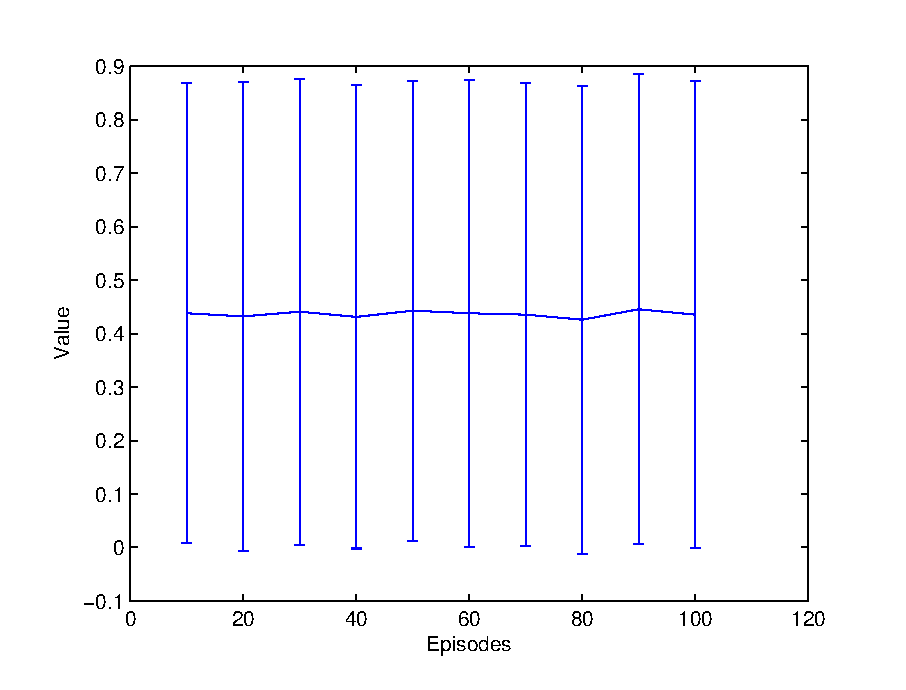
\includegraphics[width=8cm]{figures/django1vs1.eps}\	
    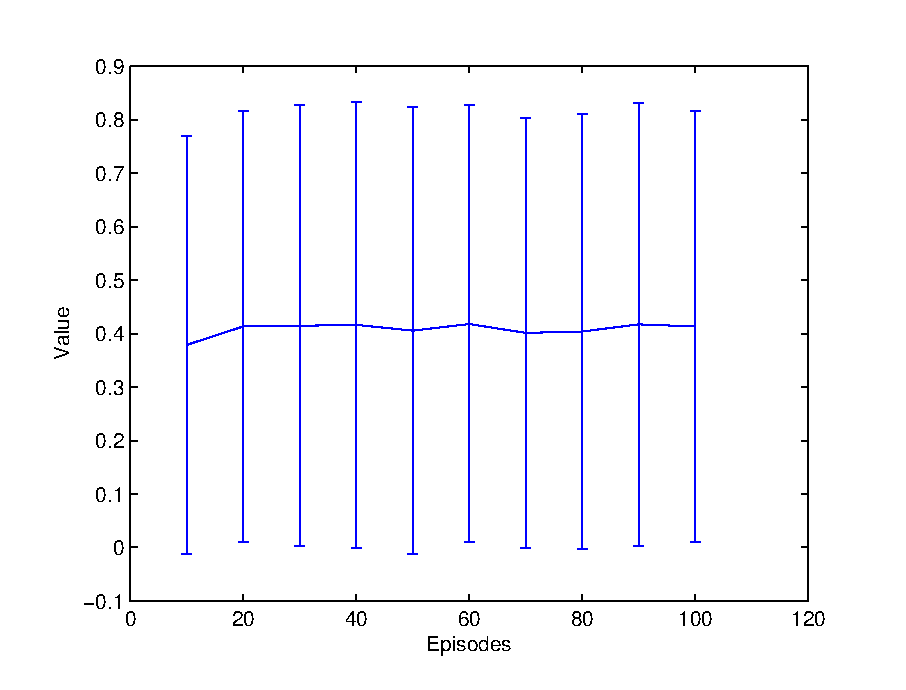
\includegraphics[width=8cm]{figures/django3vs3.eps}
   \caption{Experimental results. Left, $1vs1$ agents setting. Right, $3vs3$ agents setting.}
   \label{django}
\end{figure*}

\subsection{Interesting Points as States}
In the previous subsection, we described an easy way to formalize the problem of learning in this Markov decision process setting. Our approach for selecting an ideal state and action space was not really applicable to this game. In this subsection, we are presenting a better way to represent the state and the action space.
\subsubsection{State-Action Space}
In \textit{Domination Game}, there are four important points in the map, the two control points and the two ammo spots. Furthermore, the initial positions of the agents can be described as an important point as well. Here, we are investigating the use of these important spots into the map as states in the MDP representation of our learning problem. Hence the feature describing the position is an important point of the map. This can be described as:
\begin{equation}
S_{position} = \lbrace CP_1, CP_2, AM_1, AM_2, INIT  \rbrace
\end{equation}
But, this is a really minimalistic representation in contrast to the previous one, which had a grid over all map positions. So, we decided to represent a joint state space which includes information for all the three agents. Agents now, will decide their action not only depending on their own locations, but also on where their teammates are located.
\begin{equation}
S'_{position} = S_{position} \times S_{position} \times S_{position}
\end{equation}
The first position in this product is always referring to the agent who updates its \textit{Q-table}, and the other two positions are referring to the other two agents in lexicographic order.

The current position state of each agent is given always by its previous visited state in this state space and the action is represented by the driving goal of the agent. We also used the state of the control points as they were described in equation (3). Third component of our state space is the opponents' positions. However, our agents are not always aware of the opponents' positions in the map, due to the limited range they can observe. As a result, we decided to represent our knowledge about the opponents as a vector of four elements, as many as the interesting points in the map except from our initial position. Each element in this vector can take integer values from $0$ to $3$, representing how many opponent agents are located near to each state.
\begin{equation}
S_{foes} = \lbrace <0,0,0,0>, <0,0,0,1>, \ldots, <0,0,0,3>  \rbrace
\end{equation}
The knowledge of the opponents' positions is known to all of our agents, even if only one agent of our team can see opponents.

The possible actions of each agent were to drive in one of the possible points of interest, and/or shoot.
The action set was:
\begin{equation}
A = \lbrace CP_1, CP_2, AM_1, AM_2 \rbrace
\end{equation}
The state-action space is now:
\begin{equation}
S = S'_{position} \times S_{full\_cps} \times S_{foes} \times A
\end{equation}
Comparing with the previous approach described in the above subsection, we can realize that this one is more compact and it allows to us use more information.
\subsubsection{Reward Function}
The reward function is the same as described in the grid world approach.
\subsubsection{Learning Method}
Once more, we decided to implement \textit{independent Q-Learning} for each one of our agents. Now, each agent does not keep its own \textit{Q-table}, but all agents update the same joint Q-table. We can see it as a group of agents try to learn a symmetric optimal policy. As an example, imagine there are two agents in states A,B respectively. The optimal action for agent one, in state A and agent two in state B, is the same as the optimal action for the second agent in state A and agent one in state B. Again, the update rule of the \textit{Q-Learning}, updates the table of each independent agent every time the agent reaches its target state, i.e. its previous action. We used \textit{Q-Learning} with $0.7$ learning rate-$\alpha$ and the same value for discount factor-$\gamma$.
\begin{figure*}[t]
\centering  
    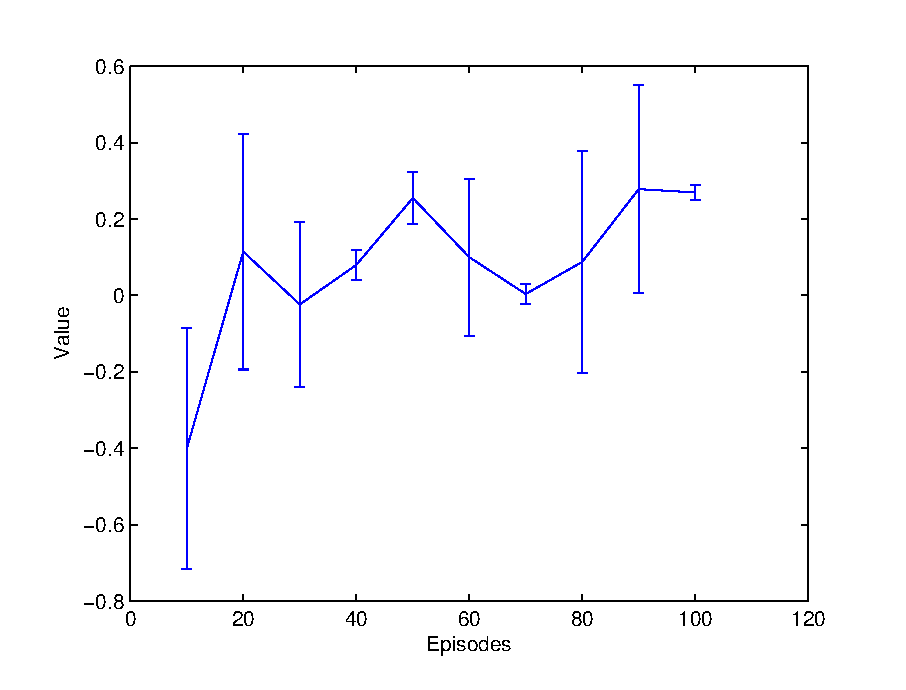
\includegraphics[width=8cm]{figures/snake1vs1.eps}\	
    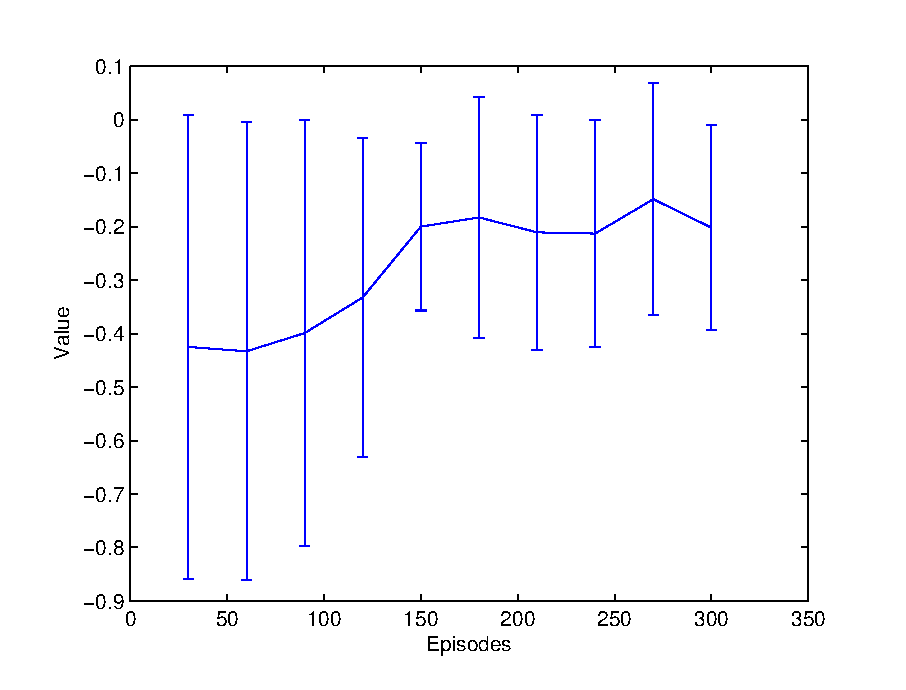
\includegraphics[width=8cm]{figures/snake3vs3.eps}
   \caption{Experimental results. Left, $1vs1$ agents setting. Right, $3vs3$ agents setting.}
   \label{snake}
\end{figure*}
\subsubsection{Results}
Finally, the results of this approach are illustrated in the Figure~\ref{django}. We tested our approach against the random-default agent. The value represented by the y-axis in these figures is:
\begin{equation}
step = (max\_steps - end\_steps)/ max\_steps
\end{equation}
\begin{equation}
score = (score - max\_score/2)/max\_score
\end{equation}
\begin{equation}
value = step \times score
\end{equation}

From the last three equations, we can refer that a win counts more if it is early in respect to the total steps that the game can continue, and a lost in the lately steps is better than a lost one in the early steps. We tune the settings of the game, and these episodes last for $3000$ steps, and the maximum score is $1000$, in order to have a faster learning process. In every number of episodes in the x-axis the average of the previous $10$ episodes is computed. The whole simulation repeated three times, the mean and the standard deviation are presented. The left graph in figure~\ref{django}, is about an one vs. one game. We can see that our learning agent obtains a high reward even from the first ten completed episodes. This is normal, because the agents chooses action among only interesting points, causing to a behavior similar to the random-default agent. In addition, it learns to choose actions that are profitable for it. The same applies for the right graph, where we have a complete team of three agents against the default team. Only a small reduction of the value that the agents obtained over the first $10$ episodes is observed.


\subsection{Interesting Points and Transitions as States}
We pointed out, how the performance of our agent improved using interesting points as the state space of our MDP framework. Here, we are investigating one more improvement that can lead us to a better learning scheme.In general, considering only interesting points as states, causes significant delay in the update of the \textit{Q-table} for example. Furthermore, there might be also a lot of changes in the world state while an agent is in a transition from its previous state to another. Imagine for example, that agent A chooses an action towards the control point 1. Simultaneously, agent B chooses the same action, agent A reaches control point 1 first, but agent B cannot change its action and is forced to go to the control point no matter if it is taken by its teammate. Thus, there is a need of additional states which are going to describe transitions from one state to another. This idea is exploited through the next part of this paper, in aiming at optimal decision making.
\subsubsection{State-Action Space}
As in previous part in this section, we are going to describe each part of the MDP representation. First of all, the feature of the state space which is going to represent the position of each agent is now different. Given a set of states as in eq. (7), and a set of transitions T, the new state space will be:
\begin{equation}
S_{position} = \lbrace CP_1, CP_2, AM_1, AM_2, INIT  \rbrace
\end{equation}
\begin{equation}
T_{position} = permutations(S_{position}, S_{position})
\end{equation}
\begin{equation}
S'_{position} = chain(S_{position}, T_{position})
\end{equation}
So, the agent now, can be in state:
\begin{itemize}
\item I am in state $CP_1$ or,
\item I am going from $CP_1$ to $CP_2$.
\end{itemize}
As one can realize, this is a simple way to add more information about states. Unfortunately, the size of the new state space is already too large to contain the same amount of information for each agent in one team. So, we decided, in order to make it computationally feasible, to represent the state of our teammates with their temporal goal, again, in lexicographical order.
\begin{equation}
S''_{position} = S'_{position} \times S_{position} \times S_{position} 
\end{equation}
In this test case, we are not using the information for the opponent agents' positions, in order to contain a computationally tractable statespace, but we use the Cps states from eq. (3).

For the action space, each agent has all possible position states except for the initial positions.
The action set is the same as before.
\begin{equation}
A = \lbrace CP_1, CP_2, AM_1, AM_2 \rbrace
\end{equation}
The state-action space is now:
\begin{equation}
S = S''_{position} \times S_{full\_cps} \times A
\end{equation}
\subsubsection{Reward Function}
The reward function is the same as described in the grid world approach. This function is described in eq. (5-6).
\subsubsection{Learning Method}
The reason why we chose to implement \textit{Independent Q-Learning} not only in this test case, but in the previous test cases as well, was the fact that the state-action space then was really intractable. Almost $500Mb$ was the necessity in memory for the Q-table when we tried to include joint actions in our state and action space, which is indicative about how much the state space grows in a multi-agent setting.
Again, the update rule of the \textit{Q-Learning}, updates the table of each independent agent every time the agent reaches its target state, i.e. its previous action. We used \textit{Q-Learning} with $0.7$ learning rate-$\alpha$ and the same value for discount factor-$\gamma$. Each update rule is performed after each game-step and not like the previous case, when the update rule was only performed after each arrival in the target state.
\subsubsection{Results}
In figure~\ref{snake}, the results of the discussed approach are presented. The same values are presented here as in the previous figure for x and y axis. As it is explained before, when now agents choose an action and aim towards a future state, until this is completed they will find themselves in a transition state. From this transition state, they can also choose an action, towards another state different from their initial target. This causes poor performance on the early episodes. Again, the graph on the left represents only two agents playing against each other. After $100$ games-episodes, the learning agent obtains a value of greater than $0.2$, which is lower than the previous test case. Results are worse for the three versus three game. After a huge number of episodes, $300$, the only thing that the learning team of agents actually has learned is how to lose in more timesteps than it used to. One possible explanation is that now the state space is significantly larger, and the agents have not complete information about the opponents, and their teammates' position as in the previous test case. One possible improvement would be to include joint actions in our state-action space. Then, the policy would have been better, and the learning process would not have lead the agents to learn a symmetric optimal policy to act. However, these are difficulties that appear when dealing with huge state spaces, this framework really gave us the change to understand why learning and planning in huge state spaces is challenging, especially with the presence of multiple agents.


\section{Future Work}

In this section, we present some of the features we consider worth improving, both on theoretical basis but also regarding the strategic setup of our implementation.

\subsection{Testing vs. Learning Agents}
It is a fact that due to time constraints we did not have time to test our agents' performance opposed to every other team that competed in the tournament. For this reason, we only include testing cases using the default agent as the opponent team. We would like to observe how our agents would perform against learning agents aswell, but this was not possible since most teams' implementations included learning methods only in the last tournament.

\subsection{Higher-level Learning}
What we discuss as a "higher-level learning" concept is implementing methods in which agents do not learn regarding their next action in every discrete timestep, instead, each agent is dynamically assigned with a certain role as the game progresses. This means, that we could have a set of strategies, or roles, preset in our implementation and let them learn which role is appropriate at each stage of the DG. In that way, we could considerably reduce the statespace, which could only include the current score of a fight and the condition of the control points, and define roles for each situation (winning or losing the game so far).

\section{Conclusion}

Creating algorithms to compete in the Domination Game has been a demanding challenge. As a conclusion, it is proven to be computationally expensive to create a fully operational learning-based team of agents. Given the huge statespace, a team designed to win the tournament should definately implement preset strategies, and implement a role-learning algorithm to adapt to the opponent team. Results of the first two tournaments have shown that hand-coded strategies can be really efficient, however, adding learning methods to already well-performing strategies is a massive boost towards victory.


\begin{thebibliography}{9}

\bibitem{MARL}
L. Busoniu, R. Babuska and B. De Schutter, \emph{A Comprehensive Survey of Multiagent Reinforcement Learning}, IEEE Transactions on systems, MAN, and Cybernetics, Part C: Applications and Reviews, vol. 38, No. 2, March 2008.

\bibitem{bouzy}
B. Bouzy, M. Metivier, \emph{Multi-agent Learning Experiments on Repeated Matrix Games}, Universite de Paris.

\bibitem{mach}
F. Schweitzer and R. Mach, \emph{Distribution of Strategies in a Spatial Multi-Agent Game}, ETH Zurich.

\bibitem{strats}
E. Raboin, D. Nau,U. Kuter, S. K. Gupta and P. Svec, \emph{Strategy Generation in Multi-Agent Imperfect-Information
Pursuit Games}, University of Maryland.

\bibitem{boutilier}
C. Boutilier, T. Dean and S. Hanks, \emph{Decision-theoretic planning: Structural assumptions and computational leverage}, 2011

\end{thebibliography}


\end{document}


